\documentclass{bioinfo}
\copyrightyear{2017}
\pubyear{2017}




%%% Additional Macro and command.
\usepackage{url}
\newcommand{\pkg}[1]{{\fontseries{b}\selectfont #1}}
\makeatletter
\newcommand\code{\bgroup\@makeother\_\@makeother\~\@makeother\$\@codex}
\def\@codex#1{{\normalfont\ttfamily\hyphenchar\font=-1 #1}\egroup}
\makeatother
\let\proglang=\textsf
%%% End of additional Macro and command.

%\usepackage[doublespacing]{setspace}

\newcommand{\package}{\textbf{AnaCoDa }} % need that whitespace there for text flow
\usepackage{natbib}

%%% Start here.
\begin{document}


\firstpage{1}

\title[AnaCoDa]{AnaCoDa: Analyzing Codon Data with Bayesian mixture models}
\author[
Landerer \textit{et~al}]{Cedric Landerer\,$^{1,2}$\footnote{
to whom correspondence should be addressed
},
Alexander Cope\,$^{3,5}$
Russell Zaretzki\,$^{2,4}$, and
Michael A.~Gilchrist\,$^{1,2}$
}
\address{$^{1}$
Department of Ecology and Evolutionary Biology, University of Tennessee, Knoxville, TN, USA.
$^{2}$National Institute for Mathematical and Biological Synthesis.
$^{3}$Genome Science and Technology, University of Tennessee, Knoxville, TN, USA.
$^{4}$Department of Statistics, Operations, and Management Science,
University of Tennessee, Knoxville, TN, USA.
$^{5}$Oak Ridge National Laboratory, Oak Ridge, TN, USA.} 
\history{Received on XXXXX; revised on XXXXX; accepted on XXXXX}

\editor{Associate Editor: XXXXXXX}

\maketitle

\begin{abstract}

\pkg{\package} is a fast and reliable software for estimating biological parameters, such as selection against translation inefficiency, nonsense error rates, and ribosome pausing times, for sets of genes based on codon or amino acid scale data, such as foot print counts or amino acid frequency.
\package provides an adaptive Bayesian MCMC algorithm, fully implemented in C++ for high computational performance with an ergonomic R interface to improve usability. 
\package also follows a generic object-oriented design to allow users to extend the framework and implement their own models for analyzing biological data.
Current models within \package can accurately estimate relevant parameters given either coding sequences or ribosome foot-printing data, depending on the model.
Optionally, \package can utilize additional data sources, such as gene expression measurements, to improve model fitting and parameter estimation.
By utilizing a hierarchical object structure, some parameters can vary between sets of genes while others can be shared.
Gene membership in a set can either be pre-assigned by the user or estimated by \package itself.
This flexibility allows users to estimate the same model parameter under different biological conditions and categorize genes into different sets based on shared model properties embedded within the data.
\package also allows users to generate simulated data which can be used to aid model development and model analysis as well as evaluate model adequacy.
Finally, \package also comes with a set of visualization tools and the ability to revisit or reinitiate previous model fittings.
[SHOULD MENTION OF PARALLELIZATION]
[CONCLUSION STATEMENT NEEDED]

\section{Availability:}
\pkg{\package} is freely available under the Mozilla Public License 2.0
on CRAN (\url{http://cran.r-project.org/package=anacoda}).

\section{Contact:} \href{cedric.landerer@gmail.com}{cedric.landerer@gmail.com}
\end{abstract}


\section*{Introduction}
The exponential increase in publicly available genomes over the past decade and the addition of novel technologies produced a vast amount of data for researchers.  
This influx of raw data necessitates the development of computational tools for extracting biological information. 
Models have to be developed and provided to the public in easy to use software to allow researchers to analyze classical sequence data as well as novel data like ribosome foot-printing counts.

Here, we describe an open-source software implemented in R \citep{rcore} that allows researchers to analyze genome-scale data like coding sequences and ribosome foot-printing data in a Bayesian framework under various models. 
\package implements an adaptive Gibbs sampler within a Metropolis-Hastings Monte Carlo Markov Chain (MCMC) approach. This allows for the incorporation of prior knowledge and easy sampling from the posterior distribution to estimate parameter values and quantify the degree of uncertainty in these estimates.
Currently, \package provides three models to analyze codon counts obtained from coding sequences or ribosome foot-printing experiments. However, \package provides a modular infrastructure such that additional genome scale or even phylogenetic models can be integrated. 
\package provides a generic, mixture distribution option to all implemented models, allowing for estimation of condition specific parameters or the automatic categorization of data into different sets based on differences in their posterior probabilities of set membership.

The \package framework works with gene level data such as codon frequencies or position specific footprint counts.
Conceptually, \package uses three different types of parameters.
The first type of parameters are gene level parameters such as gene expression level or functionality.
Gene-specific parameters are estimated separately for each gene and can vary between potential gene categories or sets.
The second type of parameters are gene set level parameters, such as mutation bias terms or translation error rates.
These parameters are shared across genes in a set and can be exclusive to a single set or shared across multiple sets.
While the number of gene sets must be pre-defined by the user, set assignment of genes can be pre-defined or estimated as part of the model fitting.
Estimation of the set assignment provides the probability of a gene being assigned to a set allowing the user to asses the uncertainty in each assignment.
The third type of parameters are hyperparameters, such as a parameters for a prior distribution for mutation bias or error rates.
Hyperparameters can be set specific or shared across multiple sets and allow for the construction and analysis of hierarchical models.
In order to reduce the effect of the 'curse of dimensionality' on the sampling efficiency of the MCMC chain and allow flexibility in parallelization, \package uses a Gibbs sampling approach where the MCMC sampling of one parameter type is conditioned on the other two types.


%\begin{figure*}[!tpb]
%\centering
% 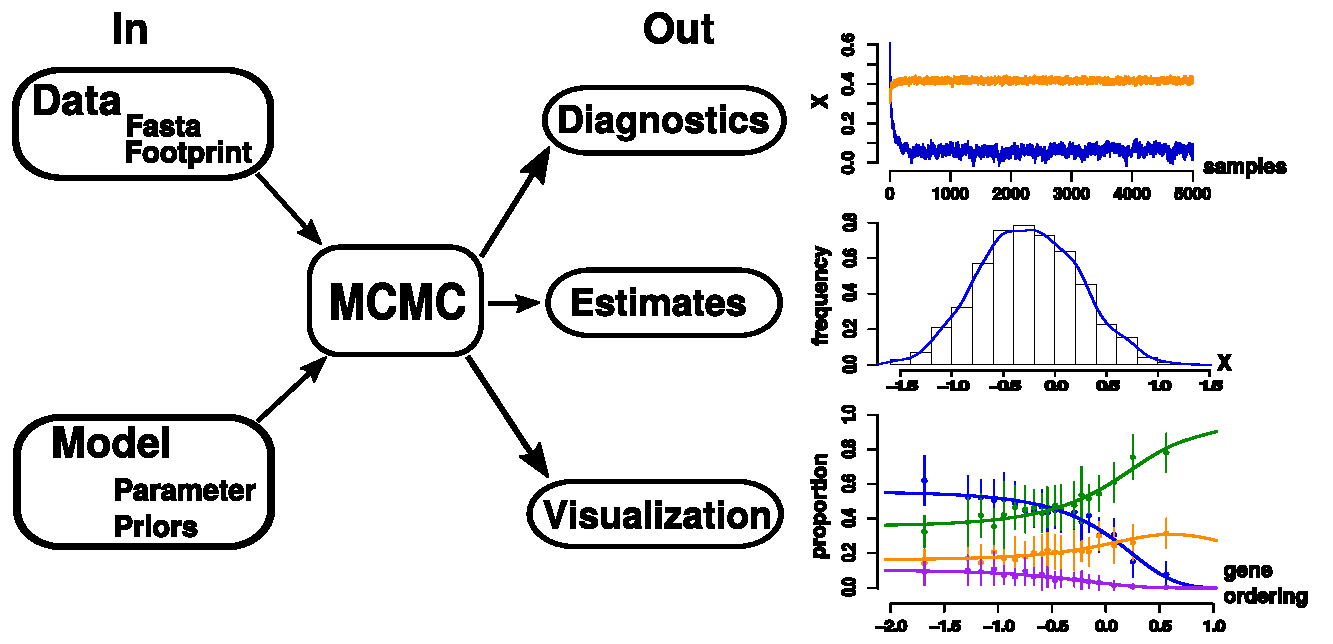
\includegraphics[width=4.5in]{workflow_croped.pdf}
%\vspace{-0.2cm}
%\caption{\textbf{Package overview and plotting functionality.} \package \textbf{Illustration of the angus workflow.} 
%\package allows for the easy estimation of population genetics parameters from genome scale data such as CDS or ribosome footprints. 
%Furthermore, \package provides functionality for MCMC diagnostics and visualization. 
%}
%\label{fig:plotbin}
%\end{figure*}

\section*{Features}
\package provides an interface written in R, a freely available programming language noted for its ease of use for even inexperienced programmers. 
As a result, \package is accessible to researchers with minimal computational experience. 

The \package interface is designed for quick and efficient data analysis.
Generally, the only input needed for fitting a model to the data are protein-coding nucleotide sequences in the form of a FASTA file or a flat-file containing codon counts obtained from ribosome foot-printing experiments. 
If available, users may also provide additional types of data such as estimates of gene expression.
\package can simultaneously utilize the information embedded in these additional data types and/or estimate the error associated with it.
\package also provides visualization functionality, including plotting functions to compare parameter estimates for different mixture distributions and display codon usage patterns (Figure 1). In addition, diagnostic functions such as those for calculating and visualizing the degree of autocorrelation in MCMC samples are provided.

\subsubsection*{Robust and efficient model fitting}
\package has built-in features designed to improve the robustness and performance of the implemented MCMC approach. 
For example, the implemented MCMC approach automatically adapts the proposal width for sampled parameters, improving sampling efficiency of the MCMC and computational performance.
Even though \package is written in C++, analysis of large datasets and/or complex models can be very computationally intensive.
In order to protect users from computer failures or aid in the collection of additional MCMC samples, \package periodically produces output files which can be used to restart an MCMC chain from a previous time point.
In addition, \package is capable of thinning the MCMC chain, meaning only every $k^{th}$ sample is kept. 
Thinning increases the effective number of samples by reducing the auto-correlation between samples and reduces the amount of memory required by the underlying data structures. 
\package is also able to create file R compatible representations of its parameter and MCMC objects.
These objects can be loaded into the R environment for model analysis and visualization.

Although \package is provided as an R package, the main computational work is implemented in C++ and can be, if desired, compiled as a standalone software.
Because R does not provide native C++ support, we used the R package Rcpp which allows for the exposure of whole C++ classes as modules to R \citep{rcpp_package}.
Using Rcpp eliminates time consuming data transfer between the R environment and the C++ core during runs, resulting in improved computational performance and allowed for a fully object-oriented code design \cite{ood_book}. 
As expected, the runtime of \package scales linear with genome size and number of iterations, and polynomial with the number of mixture distributions in the data set. The polynomial increase in the number of mixture distributions is explained by the necessity to estimate the protein production rate for each gene in each mixture distribution, as it is a gene specific parameter and the probability of a gene being assigned to a mixture has to be conditioned on it.



%\subsubsection*{Mixture distributions}
%[IT SEEMS LIKE THIS SECTION SEEMS A BIT REDUNDANT WITH PREVIOUS DISCUSSION OF MIXTURES.
%IS IT NEEDED?  
%CAN THE REDUNDANCY BE REDUCED WHILE THE FEATURE BE BETTER SOLD?
%ALSO, ROC MODEL IS INTRODUCED HERE BUT ONLY REFERENCED AND DEFINED LATER.
%]
%Mixture distributions are commonly used when a data set is comprised of sub-populations or sets which can be described by mixing various distribution \citep{gelman2013}. 
%\package allows all implemented models with the ability to utilize mixture distributions for all set specific parameters like codon specific mutation and selection bias in the case of the ROC model. 
%The separation of gene specific and set specific parameters creates the necessity to estimate a gene specific parameter for each possible set a gene can be assigned to. 
%This approach allows genes to be categorized based on differences in set specific parameters, like codon-specific mutation and selection biases, making \package ideal to ask questions about intra-genomic or even within-gene heterogeneity in mutation and selection patterns (see Landerer et al. XXXX for application [SHOULD IDEALLY HAVE A REFERENCE TO YOUR PAPER ON bioRXiV). 


\subsubsection*{Data Simulation}
In addition to model fitting to actual datasets, \package can be used to generate simulated data sets as well.
On their own, simulated datasets are useful for model development and analysis.
Simulating data under different conditions allows the user to explore model behavior. 
Different conditions can include the addition or elimination of parameters, or simply allowing a set of parameter values to vary.
Fitting models to simulated data can provide users insight into potential pitfalls or shortcomings when fitting observational data and can serve as the basis for evaluating model adequacy of a model fit to observational data \citep{gumi2015}.
Significant differences between the simulated and observational data suggests the current set of parameters or the model as a whole fail to include or adequately represent biological mechanisms underlying the observational data.
 
\subsubsection*{Available models}
\package currently provides codon models for analyzing genome scale data.
The ROC model extends the codon usage bias model developed by \citet{gilchrist2015,wallace2013,shah2011}, which can reliably estimate the strength of selection on \underline{r}ibosome \underline{o}verhead \underline{c}ost, mutation bias and allows for the inference of protein synthesis rates.

This model allow for the separation of effects of mutation and selection based on gene ordering by protein synthesis rate, and the added mixture distribution allows for gene clustering based on these effects.
Furthermore, \package implements a ribosome PAusing (PA) model to estimate codon specific ribosome pausing times from ribosome foot-printing data.

%\subsubsection*{User Defined Models}
%\package defines an interface to connect models with the implemented MCMC algorithm. 
%Implementing this interface allows researchers to add their own models to analyze sequence, foot-printing data or other data-types.
%Researchers are able to create their own models, implementing the provided interface and inheriting functionality shared with other models.
%Functionality unique to a model must be contained within the new model. 
%[THIS IS PROBABLY THE MOST POORLY WRITTEN SECTION]


\bibliographystyle{natbib}
\bibliography{bioinfo}
\end{document}
